\begin{frame}{Introduction to SoCRocket}
\begin{block}{Basic Problem}
  \begin{itemize}
		\item Increasing transistor density on die influences commercial and aerospace domain 
			\begin{itemize}
				\item System-on-Chip (SoC) gets more complex
				\item More efficient utilization of the silicon
			\end{itemize}
			\item Gained chip capacity is not fully usable
			\item Hardware-Software-productivity gap	
	\end{itemize}
\end{block}
\end{frame}

\begin{frame}{Hardware-Software-productivity gap}
	\begin{figure}
	\label{fig:prodgap}
	\centering
	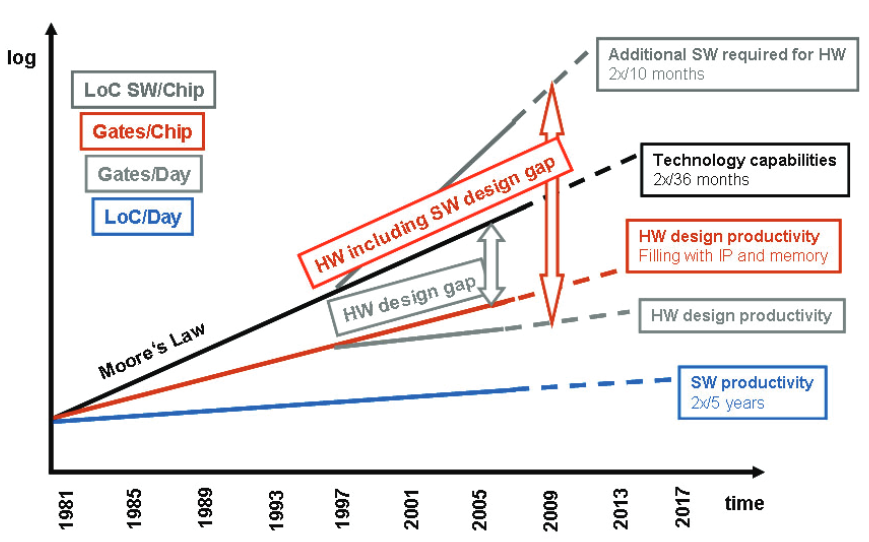
\includegraphics[width=0.9\textwidth]{pictures/Productivity.PNG}
	\end{figure}
	ITRS Roadmap 2007\footnote{\url{https://www.semiconductors.org/wp-content/uploads/2018/08/2007Design.pdf)}}
\end{frame}


\begin{frame}{Introduction to SoCRocket}
\begin{block}{Solution}
  \begin{itemize}
		\item Raise of abstraction level
			\begin{itemize}
				\item VHDL and Verilog in the 1990s
				\item	Re-Using RTL IP-cores \& enabling more on-chip memory is the standard 
				\item	SystemC and Transaction Level Modelling (TLM) are new approaches
			\end{itemize}
		\item Pros and Cons
			\begin{itemize}
				\item + Better overview of the whole architecture
				\item + Enable simpler early software design
				\item - Lack of simulation environments
				\item - Missing experts
			\end{itemize}
		\end{itemize}
\end{block}
\end{frame}


\begin{frame}{Introduction to SoCRocket}
\begin{block}{Overview}
  \begin{itemize}
		\item The SoCRocket Open Virtual Platform enables high abstraction models
		\item Goal: Animate industry to use TLM
		\item Solve past problems by making the whole platform open
			\begin{itemize}
				\item No standardization
				\item New workflows
			\end{itemize} 
		\item Based on enclosure of system basic functionalities 
		\item Library basic classes bequest functionalities
	\end{itemize}
\end{block}
\end{frame}


\begin{frame}{Introduction to SoCRocket}
\begin{block}{Content of SoCRocket}
  \begin{itemize}
		\item Contains a library of IP-Core models especially for the aerospace domain
		\item IP-cores provided by 
			\begin{itemize}
				\item European Space Agency (ESA)
				\item Aeroflex Gaisler with GR-LIB
			\end{itemize}
		\item Also contains variety of SystemC simulation models
	\end{itemize}
\end{block}
\end{frame}